% Options for packages loaded elsewhere
\PassOptionsToPackage{unicode}{hyperref}
\PassOptionsToPackage{hyphens}{url}
%
\documentclass[
  10pt,
]{article}
\usepackage{amsmath,amssymb}
\usepackage{iftex}
\ifPDFTeX
  \usepackage[T1]{fontenc}
  \usepackage[utf8]{inputenc}
  \usepackage{textcomp} % provide euro and other symbols
\else % if luatex or xetex
  \usepackage{unicode-math} % this also loads fontspec
  \defaultfontfeatures{Scale=MatchLowercase}
  \defaultfontfeatures[\rmfamily]{Ligatures=TeX,Scale=1}
\fi
\usepackage{lmodern}
\ifPDFTeX\else
  % xetex/luatex font selection
\fi
% Use upquote if available, for straight quotes in verbatim environments
\IfFileExists{upquote.sty}{\usepackage{upquote}}{}
\IfFileExists{microtype.sty}{% use microtype if available
  \usepackage[]{microtype}
  \UseMicrotypeSet[protrusion]{basicmath} % disable protrusion for tt fonts
}{}
\makeatletter
\@ifundefined{KOMAClassName}{% if non-KOMA class
  \IfFileExists{parskip.sty}{%
    \usepackage{parskip}
  }{% else
    \setlength{\parindent}{0pt}
    \setlength{\parskip}{6pt plus 2pt minus 1pt}}
}{% if KOMA class
  \KOMAoptions{parskip=half}}
\makeatother
\usepackage{xcolor}
\usepackage[top=2cm,bottom=1.5cm,left=1.5cm,right=1.5cm]{geometry}
\usepackage{longtable,booktabs,array}
\usepackage{calc} % for calculating minipage widths
% Correct order of tables after \paragraph or \subparagraph
\usepackage{etoolbox}
\makeatletter
\patchcmd\longtable{\par}{\if@noskipsec\mbox{}\fi\par}{}{}
\makeatother
% Allow footnotes in longtable head/foot
\IfFileExists{footnotehyper.sty}{\usepackage{footnotehyper}}{\usepackage{footnote}}
\makesavenoteenv{longtable}
\usepackage{graphicx}
\makeatletter
\def\maxwidth{\ifdim\Gin@nat@width>\linewidth\linewidth\else\Gin@nat@width\fi}
\def\maxheight{\ifdim\Gin@nat@height>\textheight\textheight\else\Gin@nat@height\fi}
\makeatother
% Scale images if necessary, so that they will not overflow the page
% margins by default, and it is still possible to overwrite the defaults
% using explicit options in \includegraphics[width, height, ...]{}
\setkeys{Gin}{width=\maxwidth,height=\maxheight,keepaspectratio}
% Set default figure placement to htbp
\makeatletter
\def\fps@figure{htbp}
\makeatother
\setlength{\emergencystretch}{3em} % prevent overfull lines
\providecommand{\tightlist}{%
  \setlength{\itemsep}{0pt}\setlength{\parskip}{0pt}}
\setcounter{secnumdepth}{-\maxdimen} % remove section numbering
\usepackage{amsmath}
\usepackage{amssymb}
\usepackage{booktabs}
\usepackage{xcolor}
\usepackage{xfrac}
\usepackage{stackrel}
\usepackage{cancel}
\usepackage{tikz}  % per \foreach
\usepackage{layout}
\usepackage{array}
\usepackage{fancyhdr}
\pagestyle{fancy}
\usepackage{comment}
\usepackage{fancyhdr}
\usepackage{float}



\pagestyle{fancy} % Imposta lo stile fancy come predefinito

% Definisci uno stile di pagina senza numeri
\fancypagestyle{senzanumero}{%
  \fancyhf{} % Pulisce intestazione e piè di pagina
}


\fancyhf{}
\lhead{\textbf{Compito di Statistica (CLEAM)}}
\cfoot{\thepage}
\usepackage{etoolbox}
\excludecomment{sol} 
\definecolor{mygray}{gray}{0.6}

%\pagestyle{empty}

\newcommand{\quadratini}[1]{%
  \foreach \i in {1,...,#1}{%
    \fcolorbox{mygray}{white}{\phantom{\huge A}}%
    \hspace{0.5em}%
  }%
}

\newcommand{\anagrafica}{%
 % \vspace{-14cm}
  {\sffamily % font sans-serif attivo
  {Compilare in Stampatello}\\[0.5em]
  \begin{tabular}{>{\sffamily}r l}
    COGNOME: & \quadratini{18} \\[0.5em]
    NOME: & \quadratini{18} \\[0.5em]
    Matricola: & \quadratini{8} \\[0.5em]
    %Codice: & \texttt{#1} \\
  \end{tabular}\\
  \vspace{-.5cm}
  \noindent\rule{\textwidth}{0.4pt}
  } % chiusura \sffamily
}
\ifLuaTeX
  \usepackage{selnolig}  % disable illegal ligatures
\fi
\usepackage{bookmark}
\IfFileExists{xurl.sty}{\usepackage{xurl}}{} % add URL line breaks if available
\urlstyle{same}
\hypersetup{
  hidelinks,
  pdfcreator={LaTeX via pandoc}}

\author{}
\date{\vspace{-2.5em}}

\begin{document}

\vspace*{-1.4cm}
\anagrafica{}

\thispagestyle{fancy}
\fancypagestyle{firstpage}{%
  \lhead{\textbf{Prova di Statistica (CLEAM)}}
  \rhead{\texttt{6DP7XAS4HYKRJVU}}
  \cfoot{} % Rimuove il numero di pagina
}
\pagestyle{firstpage}

\subsubsection{Esercizio 1}\label{esercizio-1}

Su un campione di \(220\) imprese della provincia di Milano è stato
rilevato il bilancio, espresso in migliaia di euro, del 2020. Qui di seguito i dati raccolti in classi
e le frequenze percentuali.

\begin{sol}

\begin{table}[H]
\centering
\begin{tabular}{rrr}
\toprule
$[\text{x}_j,$ & $\text{x}_{j+1})$ & $f_{j\%}$\\
\midrule
0.0 & 1.5 & 2.727\\
1.5 & 3.0 & 40.000\\
3.0 & 5.0 & 34.091\\
5.0 & 10.0 & 23.182\\
 &  & 100.000\\
\bottomrule
\end{tabular}
\end{table}

\end{sol}

1.a (pt\hspace{.1em}4.3/31) Individuare la classe modale.

\begin{sol}

\begin{table}[H]
\centering
\begin{tabular}{rrrrrrr}
\toprule
$[\text{x}_j,$ & $\text{x}_{j+1})$ & $n_j$ & $f_j$ & $b_j$ & $h_j$ & $F_j$\\
\midrule
0.0 & 1.5 & 6 & 0.0273 & 1.5 & 1.818 & 0.0273\\
1.5 & 3.0 & 88 & 0.4000 & 1.5 & 26.667 & 0.4273\\
3.0 & 5.0 & 75 & 0.3409 & 2.0 & 17.046 & 0.7682\\
5.0 & 10.0 & 51 & 0.2318 & 5.0 & 4.636 & 1.0000\\
 &  & 220 & 1.0000 & 10.0 &  & \\
\bottomrule
\end{tabular}
\end{table}

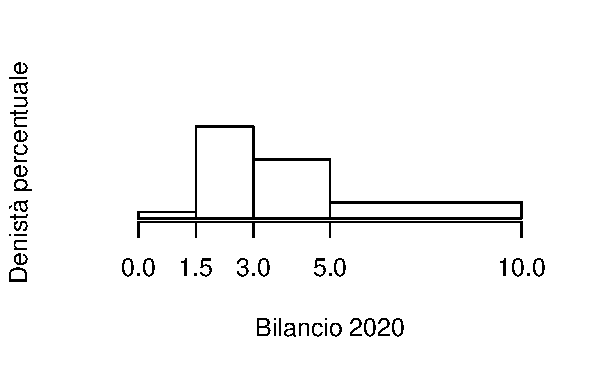
\includegraphics{www/compito_files/figure-latex/2022-80-1.pdf}

\end{sol}

1.b (pt\hspace{.1em}0.9/31) Quante imprese hanno un bilancio compreso tra \(-4\) mila
euro e zero.

\begin{sol}
\[\#(-1<X<0)=\frac{(0-(-4))26.6667}{100}\times 220=0\]

\end{sol}

1.c (pt\hspace{.1em}0.6/31) La media è risultata essere \(\bar x=3.9865\); che
relazione mi devo aspettare tra mediana e moda?

\begin{sol}
\[\bar x<x_{0.5}<x_{Mo}\]

\end{sol}

1.d (pt\hspace{.1em}0.6/31) Siano \(x_1,...,x_n\), \(n\) numeri, \(n\) dispari.
Si consideri la funzione:
\[g(x)=|x_1-x|+...+|x_n-x|.\]
Per quale valore di \(x\), \(g(x)\) è minima?

\begin{sol}
La funzione \(g\) è minimizzata nel valore della mediana.
\[x_{0.5}=x_{((n+1)/2)}\]

\end{sol}

\subsubsection{Esercizio 2}\label{esercizio-2}

Una moneta perfetta viene lanciata 5 volte, se esce almeno 3 volte testa si estrae da un'urna che contiene
un biglietto vincente ed uno perdente, altrimenti si estrae da un'urna che contine due biglietti vincenti e tre perdenti.

2.a (pt\hspace{.1em}4.3/31) Qual è la probabilità di vincere?

\begin{sol}
\begin{eqnarray*}
  P(X=3) &=& 0.1323\\
  P(X=4) &=& 0.0284\\
  P(X=5) &=& 0.0024\\
  P(X\ge 3)  &=& 0.5\\
  P(\text{Vincere})&=& 0.5\frac12+(1-0.5)\frac23\\
  &=& 0.5833
\end{eqnarray*}

\end{sol}

2.b (pt\hspace{.1em}0.9/31) Si ripete il gioco di sopra finché non si vince due volte. Qual è la probabilità di finire alla quarta giocata?

\begin{sol}
\[
3\times 0.5833\times (1-0.5833)^3\times 0.5833 = 0.0738
\]

\end{sol}

2.c (pt\hspace{.1em}0.6/31) Se \(X\sim \text{Pois}(2)\) e \(Y\sim\text{Pois}(1)\), è vero che
\[
X-Y\sim\text{Pois}(1)\qquad ?
\]

2.d (pt\hspace{.1em}0.6/31) Se \(X\) è una VC con supporto \{0,1,2\} e \(X\) è una VC con supporto \{-2,-1,0\}.
Qual è il supporto di \(X\times Y\)?

\[
\{-4,-2,-1,0\}
\]

\subsubsection{Esercizio 3}\label{esercizio-3}

3.a (pt\hspace{.1em}4.3/31) Un'urna contiene 4 palline numerate da 1 a 4.
Si estrae 100 volte con reinserimento e si fa la media dei 100 numeri
estratti. Qual è la probabilità che la media sia compresa tra 2.5 e 2.6?

\begin{sol}
\begin{eqnarray*} \mu &=& E(X_i) = \sum_{x\in S_X}x P(X=x)\\ 
 &=&  1  \frac { 1 }{ 4 }+ 2  \frac { 1 }{ 4 }+ 3  \frac { 1 }{ 4 }+ 4  \frac { 1 }{ 4 } \\ 
            &=& 2.5 \\ 
 \sigma^2 &=& V(X_i) = \sum_{x\in S_X}x^2 P(X=x)-\mu^2\\ 
 &=&\left(  1  ^2\frac { 1 }{ 4 }+ 2  ^2\frac { 1 }{ 4 }+ 3  ^2\frac { 1 }{ 4 }+ 4  ^2\frac { 1 }{ 4 } \right)-( 2.5 )^2\\ 
            &=& 1.25 
\end{eqnarray*}
\textbf{Teorema del Limite Centrale (media VC qualunque)}

Siano \(X_1\),\ldots,\(X_n\), \(n=100\) VC IID, tc \(E(X_i)=\mu=2.5\) e \(V(X_i)=\sigma^2=1.25,\forall i\), posto:
\[
      \bar X=\frac{S_n}n =\frac{X_1 + ... + X_n}n
      \]
allora:\begin{eqnarray*}
  \bar X & \mathop{\sim}\limits_{a}& N(\mu,\sigma^2/n) \\
     &\sim & N\left(2.5,\frac{1.25}{100}\right) \\
     &\sim & N(2.5,0.0125)
  \end{eqnarray*}\begin{eqnarray*}
   P( 2.5 < \bar X \leq  2.6 ) &=& P\left( \frac { 2.5  -  2.5 }{\sqrt{ 0.0125 }} < \frac { \bar X  -  \mu }{ \sqrt{\sigma^2/n} } \leq \frac { 2.6  -  2.5 }{\sqrt{ 0.0125 }}\right)  \\
              &=& P\left(  0  < Z \leq  0.89 \right) \\
              &=& \Phi( 0.89 )-\Phi( 0 )\\
              &=&  0.8133 - 0.5 \\ 
              &=&  0.3133 
   \end{eqnarray*}

\end{sol}

\subsubsection{Esercizio 4}\label{esercizio-4}

4.a (pt\hspace{.1em}0.9/31) Sia \(h\) uno stimatore per theta, tale che
\[
E(h)=\theta+\frac\theta {\sqrt{ n}}
\]
\(h\) è corretto? \(h\) è asintoticamente corretto?

\begin{sol}
\(h\) \textbf{non è corretto}, infatti
\[
E(h)=\theta+\frac\theta {\sqrt{ n}}\neq\theta
\]
\(h\) \textbf{è asintoticamente corretto}, infatti
\[
\lim_{n\to\infty}E(h)=\lim_{n\to\infty}\left(\theta+\frac\theta {\sqrt{ n}}\right)=\theta+0=\theta
\]

\end{sol}

4.b (pt\hspace{.1em}0.9/31) Siano \(h_1\) e \(h_2\) due stimatori per \(\theta\), tali che:
\begin{eqnarray*}
MSE(h_1) &=&   \frac\theta n\\
MSE(h_2) &=&   \frac{2\theta} n
\end{eqnarray*}
Quale dei due stimatori è più efficiente? Perché?

\begin{sol}
\(h_1\) \textbf{è più efficiente} di \(h_2\), infatti
\begin{eqnarray*}
MSE(h_1) &=&   \frac\theta n\\
MSE(h_2) &=&   \frac{2\theta} n =2\cdot MSE(h_1)>MSE(h_1)
\end{eqnarray*}

\end{sol}

4.c (pt\hspace{.1em}0.9/31) Si sono osservati due gruppi di dati quantitativi e si è osservato, \(\hat\mu_1=10.2\) e \(\hat\mu_2=15.6\). Posto a test
\[
\begin{cases}
H_0:\mu_1=\mu_2\\
H_1:\mu_1\ne \mu_2
\end{cases}
\]
è risultato \(p_\text{value}=0.0612\). La differenza tra \(\hat\mu_1\) e \(\hat\mu_2\) è significativa? Perché?

\begin{sol}
Il \(p_\text{value}\) è maggiore di 0.05, la differenza \textbf{non è significativa} per ogni livello di significatività.

\end{sol}

\subsubsection{Esercizio 5}\label{esercizio-5}

5.a (pt\hspace{.1em}1.2/31) Su un campione di \(n = 120\) startup tecnologiche italiane, è stato chiesto se abbiano implementato misure di cybersecurity avanzate. Lo studio ha riportato che 84 startup su 120 (il 70\% del campione) hanno implementato queste misure.

Costruire un intervallo di confidenza al 95\% per \(\pi\), la quota di startup italiane che hanno implementato misure di cybersecurity avanzate.

\begin{sol}
\(1-\alpha =0.95\) e quindi \(\alpha=0.05\rightarrow \alpha/2=0.025\)

\[
  \hat\pi = \frac{S_n}n = \frac{ 84 }{ 120 }= 0.7 
\]

\begin{eqnarray*}
  Idc: & &  \hat\pi \pm  z_{\alpha/2} \times \sqrt{\frac{\hat\pi(1-\hat\pi)}{n}} \\
     & &  0.7 \pm  1.96 \times \sqrt{\frac{ 0.7 (1- 0.7 )}{ 120 }} \\
     & &  0.7 \pm  1.96 \times  0.04183 \\
     & & [ 0.618 ,  0.782 ]
\end{eqnarray*}

\end{sol}

5.b (pt\hspace{.1em}3.0/31) Un'indagine molto più ampia condotta su startup europee ha mostrato che la percentuale di startup con misure di cybersecurity avanzate è del 80\%. Testare l'ipotesi che in Italia la quota di startup con misure di cybersecurity avanzate sia uguale a quella europea contro l'alternativa che sia minore. Risolvere col \(p_\text{value}\) e confrontarlo per \(\alpha=0.1,0.05,0.01,0.001\).

\begin{sol}
\textbf{Test \(Z\) per una proporzione}

La stima
\[\hat\pi=\frac { 84 } { 120 }= 0.7  \]

\(\fbox{A}\) FORMULAZIONE DELLE IPOTESI

\[\begin{cases}
   H_0: \pi = \pi_0=0.8 \\
   H_1: \pi < \pi_0=0.8 
   \end{cases}\]

\(\fbox{B}\) SCELTA E CALCOLO STATISTICA-TEST, \(Z\)
Test Binomiale per \(n\) grande: \(\Rightarrow\) z-Test.

\begin{eqnarray*}
   \frac{\hat\pi - \pi_{0}} {\sqrt {\pi_0(1-\pi_0)/\,n}}&\sim&N(0,1)\\
   z_{\text{obs}}
   &=& \frac{ ( 0.7 -  0.8 )} {\sqrt{ 0.8 (1- 0.8 )/ 120 }}
   =   -2.739 \,.
   \end{eqnarray*}

\(\fbox{C}\) CONCLUSIONE

Il \(p_{\text{value}}\) è

\[ p_{\text{value}} = P(Z<-2.74)=0.003085 \]

\[
 0.001 < p_\text{value}= 0.003085 \leq 0.01 
\]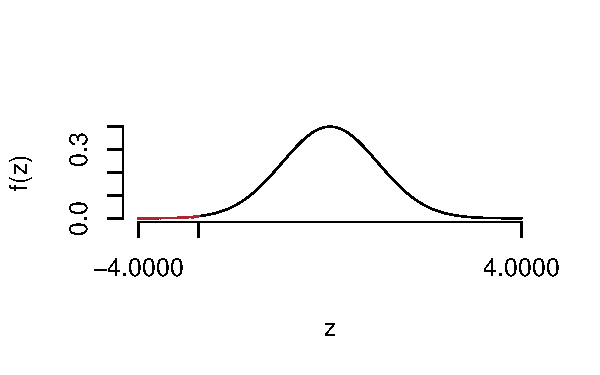
\includegraphics{www/compito_files/figure-latex/2024-130-1.pdf}

\textbf{Rifiuto} \(H_0\) all'1\%,

\(0.001<p_\text{value}<0.01\), \emph{molto significativo} \(\fbox{**}\).

\end{sol}

\subsubsection{Esercizio 6}\label{esercizio-6}

In uno studio sulla formazione aziendale, in un campione di \(n=30\) dipendenti, sono state analizzate le ore di formazione (in ore, \(X\)) e il punteggio di performance (in opportuna, \(Y\)).

Si osservano le seguenti statistiche:
\(\sum_{i=1}^{30}x_i=1036.68\), \(\sum_{i=1}^{30}y_i=538.81\),
\(\sum_{i=1}^{30}x_i^2=39787.25\), \(\sum_{i=1}^{30}y_i^2=10684.19\) e \(\sum_{i=1}^{30}x_iy_i=20527.76\).

6.a (pt\hspace{.1em}4.3/31) Si è osservato \(x_7=39.46\) e \(y_7=18.26\), stimare il modello di regressione dove \(Y\) viene spiegata da \(X\) e calcolare il residuo per il punto \(i=7\).

\begin{sol}
\begin{eqnarray*}
           \bar x &=&\frac 1 n\sum_{i=1}^n x_i = \frac {1}{ 30 }  1036.68 =  34.56 \\
           \bar y &=&\frac 1 n\sum_{i=1}^n y_i = \frac {1}{ 30 }  538.81 =  17.96 \\
           \hat\sigma_X^2&=&\frac 1 n\sum_{i=1}^n x_i^2-\bar x^2=\frac {1}{ 30 }  39787  - 34.556 ^2= 132.1 \\
           \hat\sigma_Y^2&=&\frac 1 n\sum_{i=1}^n y_i^2-\bar y^2=\frac {1}{ 30 }  10684  - 17.9603 ^2= 33.57 \\
           \text{cov}(X,Y)&=&\frac 1 n\sum_{i=1}^n x_i~y_i-\bar x\bar y=\frac {1}{ 30 }  20528 - 34.556 \cdot 17.9603 = 63.62 \\
           \hat\beta_1 &=& \frac{\text{cov}(X,Y)}{\hat\sigma_X^2} \\
                    &=& \frac{ 63.62 }{ 132.1 }  =  0.4815 \\
           \hat\beta_0 &=& \bar y - \hat\beta_1 \bar x\\
                    &=&  17.96 - 0.4815 \times  34.556 = 1.321 
         \end{eqnarray*}\begin{eqnarray*}
\hat y_i &=&\hat\beta_0+\hat\beta_1 x_i=\\ 
&=& 1.321 + 0.4815 \times 39.46 = 20.32 \\ 
\hat \varepsilon_i &=& y_i-\hat y_i\\ 
&=& 18.26 - 20.3217 = -2.062  
\end{eqnarray*}

\end{sol}

6.b (pt\hspace{.1em}0.9/31) Dare un'interpretazione dei parametri di regressione stimati.

6.c (pt\hspace{.1em}0.6/31) Perché la previsione per \(x=35\) è più affidabile di quella per \(x=346\)?

6.d (pt\hspace{.1em}0.6/31) Cosa significa che \(r\) è un numero puro?

6.e (pt\hspace{.1em}0.6/31) Se in un modello di regressione \(r=0.65\), \(\hat\sigma_X=1.1\) e \(\hat\sigma_Y=0.9\), calcolare \(\hat\beta_1\).

\begin{sol}
Per calcolare \(\hat\beta_1\) in un modello di regressione, si usa la formula:

\[
\hat\beta_1 = r \frac{\hat\sigma_Y}{\hat\sigma_X}
\]

Dati:
- \(r = 0.65\)
- \(\hat\sigma_X = 1.1\)
- \(\hat\sigma_Y = 0.9\)

Calcolo:

\[
\hat\beta_1 = 0.65 \times \frac{0.9}{1.1} = 0.65 \times 0.8182 = 0.532
\]

\end{sol}

\end{document}
